\begingroup
\linespread{1}\selectfont
\resizebox{\linewidth}{!}{%
\begin{tikzpicture}[x=1pt,y=-1pt]
\node[anchor=north west,inner sep=0pt,outer sep=0pt] at (0,0) {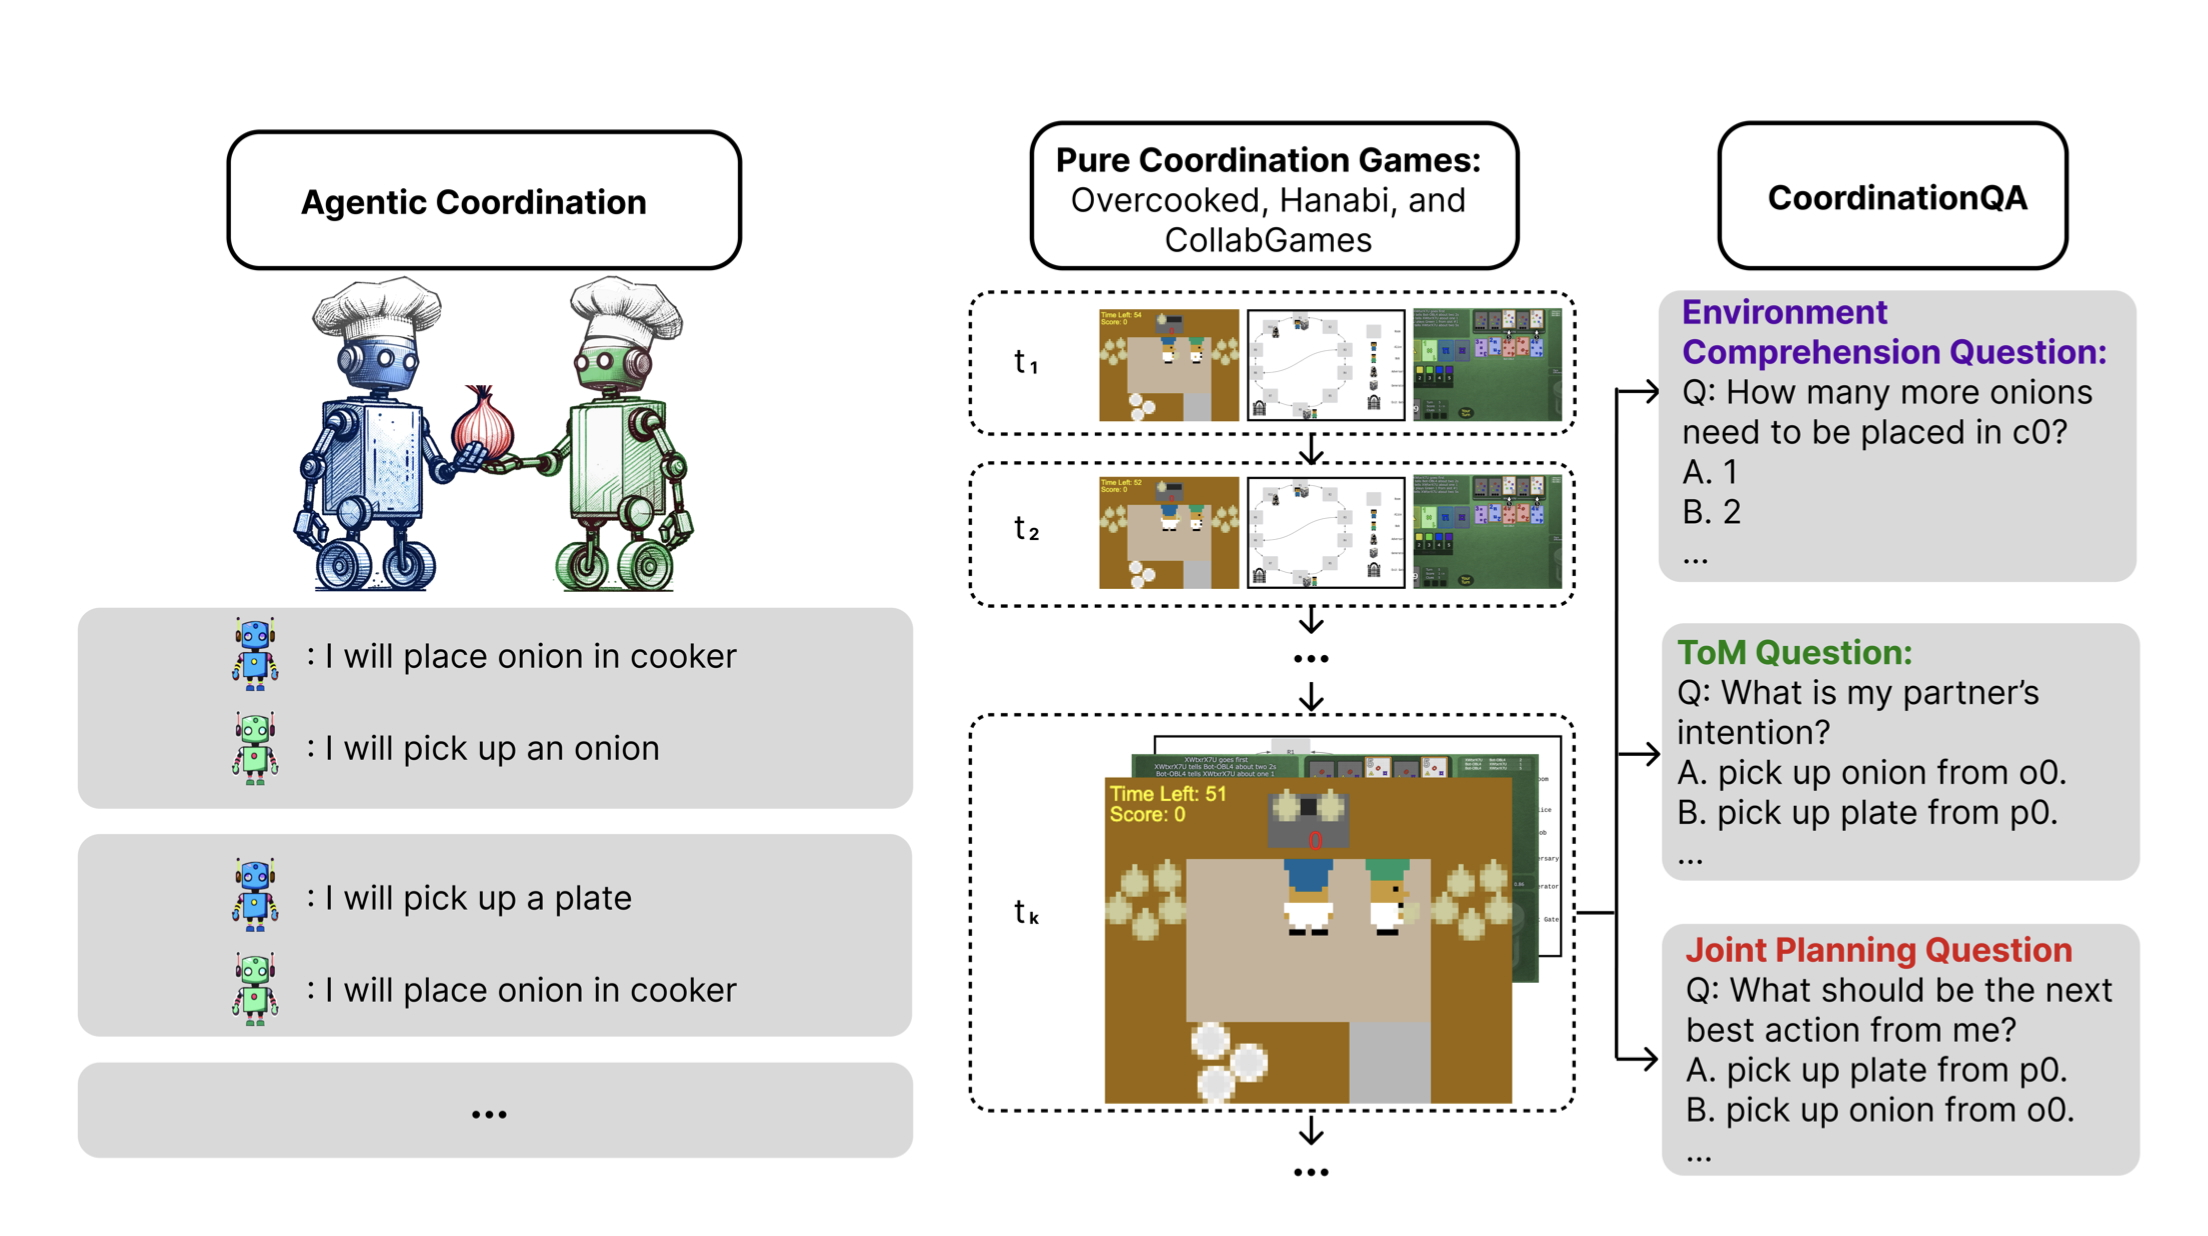
\includegraphics[width=2208pt]{figures/llmcoordinationbank.jpg}};
\fill[fill=white] (250,161) rectangle (723,244);
\node[anchor=center,inner sep=0pt,outer sep=0pt,align=center,text width=467pt,text=black,font={\fontsize{59.1429}{67.4229}\selectfont\sffamily\bfseries}] at (486.5,202.5) {智能体协调};
\fill[fill=white] (1040,133) rectangle (1510,261);
\node[anchor=center,inner sep=0pt,outer sep=0pt,align=center,text width=464pt,text=black,font={\fontsize{40.4143}{46.0723}\selectfont\sffamily}] at (1275,197) {\textbf{纯协调博弈：}\\Overcooked、Hanabi 与\\CollabGames};
\fill[fill={rgb,255:red,217;green,217;blue,217}] (305,632) rectangle (891,700);
\node[anchor=center,inner sep=0pt,outer sep=0pt,align=left,text width=580pt,text=black,font={\fontsize{44.85}{51.129}\selectfont\sffamily}] at (598,666) {：我会把洋葱放进烹饪锅。};
\fill[fill={rgb,255:red,217;green,217;blue,217}] (305,726) rectangle (891,791);
\node[anchor=center,inner sep=0pt,outer sep=0pt,align=left,text width=580pt,text=black,font={\fontsize{44.85}{51.129}\selectfont\sffamily}] at (598,758.5) {：我会取一个洋葱。};
\fill[fill={rgb,255:red,217;green,217;blue,217}] (305,877) rectangle (891,939);
\node[anchor=center,inner sep=0pt,outer sep=0pt,align=left,text width=580pt,text=black,font={\fontsize{44.85}{51.129}\selectfont\sffamily}] at (598,908) {：我会取一个盘子。};
\fill[fill={rgb,255:red,217;green,217;blue,217}] (305,972) rectangle (891,1031);
\node[anchor=center,inner sep=0pt,outer sep=0pt,align=left,text width=580pt,text=black,font={\fontsize{44.85}{51.129}\selectfont\sffamily}] at (598,1001.5) {：我会把洋葱放进烹饪锅。};
\fill[fill={rgb,255:red,217;green,217;blue,217}] (1676,295) rectangle (2125,574);
\node[anchor=north west,inner sep=0pt,outer sep=0pt,align=left,text width=429pt,text={rgb,255:red,107;green,0;blue,184},font={\fontsize{40.9071}{46.2251}\selectfont\sffamily}] at (1681,306) {\textbf{环境理解问题：}};
\node[anchor=north west,inner sep=0pt,outer sep=0pt,align=left,text width=429pt,text=black,font={\fontsize{38.4429}{43.4404}\selectfont\sffamily}] at (1681,355) {问：c0 还需放几个洋葱？\\A. 1\\B. 2\\……};
\fill[fill={rgb,255:red,217;green,217;blue,217}] (1675,634) rectangle (2124,869);
\node[anchor=north west,inner sep=0pt,outer sep=0pt,align=left,text width=429pt,text={rgb,255:red,17;green,132;blue,8},font={\fontsize{40.9071}{46.2251}\selectfont\sffamily}] at (1679,638) {\textbf{心智理论问题：}};
\node[anchor=north west,inner sep=0pt,outer sep=0pt,align=left,text width=429pt,text=black,font={\fontsize{38.4429}{43.4404}\selectfont\sffamily}] at (1679,686) {问：同伴打算做什么？\\A. 从 o0 取洋葱。\\B. 从 p0 取盘子。\\……};
\fill[fill={rgb,255:red,217;green,217;blue,217}] (1678,930) rectangle (2128,1165);
\node[anchor=north west,inner sep=0pt,outer sep=0pt,align=left,text width=432pt,text={rgb,255:red,223;green,24;blue,24},font={\fontsize{40.9071}{46.2251}\selectfont\sffamily}] at (1680,941) {\textbf{联合规划问题：}};
\node[anchor=north west,inner sep=0pt,outer sep=0pt,align=left,text width=432pt,text=black,font={\fontsize{38.4429}{43.4404}\selectfont\sffamily}] at (1680,990) {问：我的最佳下一步？\\A. 从 p0 取盘子。\\B. 从 o0 取洋葱。\\……};
\pgfresetboundingbox
\path[use as bounding box] (0,0) rectangle (2208,1236);
\end{tikzpicture}}
\endgroup
